\chapter{Исследовательская часть}

В данном разделе будут приведены примеры работы программы, и будет проведен сравнительный анализ реализованных алгоритмов по затраченному процессорному времени.

\section{Технические характеристики}

Тестирование проводилось на устройстве со следующими техническими характеристиками:

\begin{itemize}
	\item операционная система Windows 10 pro;
	\item память 32 Гб;
	\item процессор Intel(R) Core(TM) i5-12400 12th Gen 2.50 ГГц.
\end{itemize}

Тестирование проводилось на компьютере, включенном в сеть электропитания. Во время тестирования компьютер был нагружен только встроенными приложениями окружения, а также непосредственно системой тестирования.

\clearpage

\section{Демонстрация работы программы}

На рисунке \ref{img:example} приведен пример работы программы.

\begin{figure}[H]
	\begin{center}
		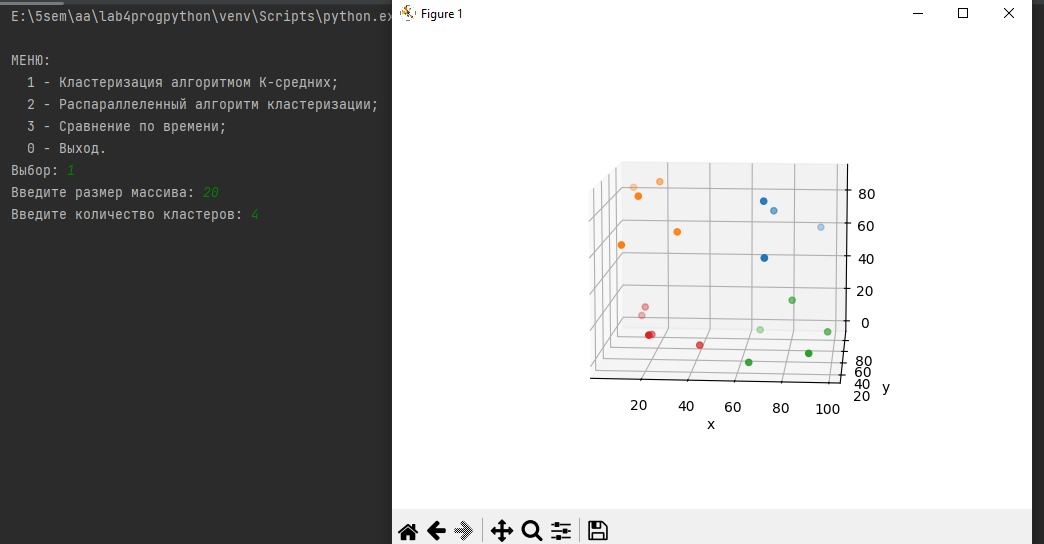
\includegraphics[scale=0.5]{img/example.png}
	\end{center}
	\captionsetup{justification=centering}
	\caption{Пример работы программы}
	\label{img:example}
\end{figure}

\section{Время выполнения алгоритмов}

Функция process\_time из библиотеки time языка программирования Python возвращает  процессорное время в секундах - значение типа float.

Для замера времени:
\begin{itemize}
	\item получить значение времени до начала выполнения алгоритма;
	\item  получить значение времени после окончания выполнения алгоритма;
	\item вычесть из второго значения первое.
\end{itemize}

Замеры проводились для массивов с исходными точками размером 100, 200, 300, 400, 500. Результаты измерения времени приведены в таблице \ref{tbl:time_even} (в мс).

\begin{table}[h]
    \begin{center}
        \begin{threeparttable}
        \captionsetup{justification=raggedright,singlelinecheck=off}
        \caption{Результаты замеров времени}
        \label{tbl:time_even}
        \begin{tabular}{|c|c|c|c|}
            \hline
            Размер & Последовательная реализация & Распараллеленная реализация \\
            \hline
		    100 & 0.0008 & 0.0003 \\ 
		    \hline
		    200 & 0.0020 & 0.0006 \\ 
		    \hline
		    300 & 0.0044 & 0.0014 \\ 
		    \hline
		    400 & 0.0059 & 0.0018 \\ 
		    \hline
		    500 & 0.0082 & 0.0028 \\ 
		    \hline
		\end{tabular}
    \end{threeparttable}
\end{center}
\end{table}



\section{Вывод}

В результате проведенного эксперимента и анализа полученных значений, можно сделать вывод,
что последовательная реализация алгоритма кластеризации методом k-средних работает медленнее распараллеленной версии
алгоритма.